%%%%%%%%%%%%%%%%%%%%%%%%%%%%%%%%%%%%%%%%%%%%%%%%%%%%%%%%%%%%%%%%%%%%%%
% How to use writeLaTeX: 
%
% You edit the source code here on the left, and the preview on the
% right shows you the result within a few seconds.
%
% Bookmark this page and share the URL with your co-authors. They can
% edit at the same time!
%
% You can upload figures, bibliographies, custom classes and
% styles using the files menu.
%
%%%%%%%%%%%%%%%%%%%%%%%%%%%%%%%%%%%%%%%%%%%%%%%%%%%%%%%%%%%%%%%%%%%%%%

\documentclass[12pt]{article}

\usepackage{sbc-template}

\usepackage{graphicx,url}

\usepackage[brazilian]{babel}   
\usepackage[T1]{fontenc} % Codificação para fontes com suporte a caracteres acentuados
\usepackage[utf8]{inputenc} % Codificação UTF-8 (necessário apenas para pdflatex)
\usepackage{multicol}
\usepackage{amsmath,amssymb,amsfonts}
\usepackage{algorithmic}
\usepackage{textcomp}
\usepackage{enumerate}
\usepackage{multirow}
\usepackage{soul}
\usepackage{verbatim}
\usepackage[table,xcdraw]{xcolor}
\usepackage[shortlabels]{enumitem}
\usepackage{scalefnt} % pacote para diminuir fonte das tabelas
\usepackage{comment} % pacote de comentarios
\usepackage{lscape}
\usepackage{fancyhdr}
\usepackage{IHC}
\usepackage[super]{nth}
\usepackage{pdfcomment}
\usepackage{float}
\usepackage{xurl}
\usepackage{booktabs}
\usepackage{array}

\sethlcolor{yellow} % highlight color used to mark revisions made in response to reviewers
\newcommand{\hlcite}[1]{\colorbox{yellow}{\cite{#1}}} % highlighted citation (soul's \hl breaks on \cite)


%By IHC 2026: package to insert description in images | pacote para inserir descrição nas imagens

%previne hifenização
\tolerance=1
\emergencystretch=\maxdimen
\hyphenpenalty=10000
\hbadness=10000

\sloppy

\input{IHC_info}

\title{Interação Humano-Dados em Contextos Urbanos: Uma Revisão Sistemática da Literatura} %deve ser no mesmo idioma do texto

\author{Autor anônimo 1, Autor anônimo 2}

\address{Endereço anônimo\\
  Estado anônimo -- País anônimo
  \email{Endereço eletrônico anônimo 1, Endereço eletrônico anônimo 2}}


\begin{document} 

%%  ATENÇÃO: AS INFORMAÇÕES DESTACADAS EM AZUL SÃO APENAS PARA INFORMAR OS AJUSTES NO TEMPLATE DA SBC E ACRESCENTAR INSTRUÇÕES DE ACESSIBILIDADE. O SEU TEXTO NÃO DEVE ESTAR NA COR AZUL.

\maketitle

\thispagestyle{plain}

%CAMPO OBRIGATÓRIO NESTE FORMATO.
\begin{abstract}{
\hl{Smart cities' growing datafication demands urban systems that respect citizen privacy and autonomy. Human-Data Interaction (HDI) addresses this gap by ensuring legibility, agency, and negotiability over digital traces. This paper presents a Systematic Literature Review (SLR), following the PRISMA protocol, mapping HDI's evolution in urban contexts across five databases (2014--2024) and yielding a final \textit{corpus} of 102 studies. Results show the field transitioning from a technical view to sociotechnical complexity, yet structural gaps persist: the lack of operational guidelines for novice designers, cognitive overload in consent management, and the neglect of ethnic-cultural factors. We conclude that HDI is fundamental for democratic urban governance, requiring data physicalization and storytelling to mitigate digital asymmetries. This mapping consolidates a baseline for future empirical work, directly advancing Grand Research Challenge GC5 (Human-Data Interaction, Data Literacy, and Usable Privacy) of the GranDIHC-BR-2025-2035 agenda.}}
\end{abstract}

\keywords{Human-Data Interaction (HDI), Smart Cities, Data Governance, Data Privacy, Data Literacy.}
     

%ATENÇÃO PESSOAS AUTORAS
\begin{resumo}{
  \hl{A dataficação crescente em cidades inteligentes exige sistemas urbanos que respeitem a privacidade e a autonomia do cidadão. A Interação Humano-Dados (IHD) responde a essa demanda garantindo legibilidade, agência e negociabilidade sobre rastros digitais. Este artigo apresenta uma Revisão Sistemática da Literatura (RSL), seguindo o protocolo PRISMA, mapeando a evolução da IHD em contextos urbanos em cinco bases de dados (2014--2024), com \textit{corpus} final de 102 trabalhos. Os resultados evidenciam a transição de uma visão técnica para a complexidade sociotécnica, mas persistem lacunas estruturais: a carência de diretrizes operacionais para projetistas novatos, a sobrecarga cognitiva na gestão de consentimentos e a negligência de fatores étnico-culturais. Conclui-se que a IHD é fundamental para uma governança urbana democrática, demandando fisicalização de dados e narrativas (\textit{storytelling}) para atenuar assimetrias digitais. Este mapeamento consolida um referencial para futuras investigações empíricas, avançando diretamente o Grande Desafio de Pesquisa GC5 (Interação Humano-Dados, Alfabetização em Dados e Privacidade Utilizável) da agenda GranDIHC-BR-2025-2035.}}
\end{resumo}

\palavraschave{Interação Humano-Dados (IHD), Cidades Inteligentes, Governança de Dados, Privacidade de Dados, Letramento de Dados.}


\section{Introdução}

    \hl{A urbanização tem avançado rapidamente ao longo do século XXI}, com projeções da ONU indicando que mais de 60\% da população global viverá em cidades,\footnote{https://brasil.un.org/pt-br/188520-onu-habitat-população-mundial-será-68-urbana-até-2050} impulsionando a busca por soluções inteligentes e sustentáveis. Em resposta a essa demanda, a comunidade científica, a indústria e a esfera política \hl{passaram a tratar} as Cidades Inteligentes (\textit{Smart Cities}) como prioridade \cite{EREMIA2017}. Esses ecossistemas utilizam tecnologias como Internet das Coisas (IoT) e Urbanismo de Plataforma, frequentemente com \textit{smartphones} atuando como sensores passivos, para otimizar serviços urbanos essenciais. \hl{Essa mesma infraestrutura, no entanto, enfrenta} desafios críticos de privacidade e segurança devido à coleta massiva (dataficação), muitas vezes realizada sob a premissa de um consentimento presumido, sem transparência ou controle efetivo pelos cidadãos \cite{streitz2019beyond}.

   Diante dessa assimetria estrutural, o paradigma da Interação Humano-Dados (IHD) surge como uma abordagem ética e centrada no usuário para reequilibrar a relação entre indivíduos e sistemas invisíveis, apoiando-se nos pilares de legibilidade, agência e negociabilidade propostos por \hlcite{mortier2015humandatainteractionhumanface}\hl{, detalhados na Seção~}\ref{sec:referencial}\hl{.}

    Apesar de o arcabouço da IHD se apresentar na literatura como uma perspectiva promissora para o reequilíbrio dessas dinâmicas, sua aplicação empírica enfrenta limitações práticas e socioculturais expressivas \cite{Victorelli2020Human}\hl{, persistentes mesmo em estudos recentes conduzidos em contextos conectados} \hlcite{DOWTHWAITE2024} \hl{e comunitários} \hlcite{hayes2024making}\hl{.} As pesquisas incorporadas a esta revisão apontam lacunas proeminentes, como a dificuldade de engajamento dos usuários leigos no \textit{design} de sistemas e a ausência de clareza em contratos de uso de dados \cite{Victorelli2020Human}. \hl{Este problema é especialmente grave para populações vulneráveis e marginalizadas, que enfrentam risco desproporcional de discriminação e exclusão diante de tecnologias orientadas a dados, muitas vezes sem letramento ou recursos suficientes para compreender plenamente as ramificações de vigilância a que estão sujeitas} \cite{malgieri2020vulnerable, hayes2024making}. Além disso, fatores contextuais intrínsecos a cada região, como disparidades culturais, letramento de dados e ambiguidades interpretativas, influenciam diretamente como os dados são gerenciados e compartilhados \cite{Yuan20243615, Belizario2023Interacao}, exigindo abordagens mais inclusivas e geopoliticamente situadas para que a interação humano-dados seja ética e transparente \cite{Elhamdadi2022}.

    Diante desse cenário, este artigo apresenta uma Revisão Sistemática da Literatura (RSL) com o objetivo de mapear como os princípios de Interação Humano-Dados (legibilidade, agência e negociabilidade) \cite{mortier2015humandatainteractionhumanface} têm sido abordados em pesquisas sobre aplicações urbanas na última década. \hl{Este trabalho mapeia o estado da arte, as tendências teóricas e as lacunas que ainda impedem uma gestão de dados mais transparente e centrada no cidadão. Os resultados desta revisão oferecem subsídios para pesquisadores e \textit{designers} de sistemas urbanos, dialogando com os Grandes Desafios de Pesquisa em Interação Humano-Computador no Brasil (GranDIHC-BR-2025-2035), em particular ao GC2 (Educação de Qualidade), ao GC3 (Governos e Cidades Inteligentes, Sustentáveis e Democráticos) e, em especial, ao GC5 (Interação Humano-Dados, Alfabetização em Dados e Privacidade Utilizável), foco central desta revisão ao investigar as lacunas de privacidade e letramento de dados em ecossistemas emergentes.}

    \hl{As principais contribuições deste artigo são: (i) uma síntese crítica da evolução histórica e conceitual da IHD entre 2014 e 2024, articulando os pilares de legibilidade, agência e negociabilidade; (ii) o mapeamento de lacunas estruturais, cognitivas e socioculturais que ainda dificultam a aplicação prática da IHD em contextos urbanos; e (iii) uma matriz comparativa de \textit{frameworks}, contextos de validação empírica e métodos de avaliação que serve de referência para trabalhos futuros na área.}

    Para o alcance dessas metas, este trabalho adota uma abordagem metodológica de natureza teórica e descritiva. O procedimento analítico foi estruturado a partir de um protocolo de mapeamento organizado em três fases fundamentais: o planejamento (delineamento das questões de pesquisa e calibração das \textit{strings} de busca), a execução (varredura nas bases de dados e aplicação dos critérios de elegibilidade) e a análise crítica (extração, categorização e síntese qualitativa das evidências), conforme detalhado na seção a seguir.
    

\section{Referencial Teórico}
\label{sec:referencial}

\hl{[Seção integralmente nova, incluída em resposta à revisão.]}

Esta seção situa, de forma sucinta, as bases conceituais nas quais esta revisão se apoia, antecipando \hl{construtos retomados} na análise crítica da Seção~\ref{sec:resultados}.

\hl{A Interação Humano-Dados (IHD) foi proposta em 2015 como um campo autônomo, distinto da Interação Humano-Computador (IHC) clássica, por deslocar o foco da usabilidade de interfaces visíveis para a relação ética entre o indivíduo e seus rastros de dados processados de forma frequentemente invisível} \hlcite{mortier2015humandatainteractionhumanface}. \hl{Esse marco fundacional é adotado nesta revisão como o divisor temporal entre o período ``pré-IHD''} \hlcite{Mashhadi2014} \hl{e a emergência da área como campo interdisciplinar próprio} \hlcite{Sailaja2021Designing}, \hl{distinção diretamente relacionada à Questão de Pesquisa QP4.}

O modelo estrutura-se em três pilares que orientam a análise desta RSL: a \textbf{legibilidade}, entendida como a capacidade do usuário de compreender e construir sentido (\textit{sensemaking}) sobre os dados coletados e os algoritmos que os processam; a \textbf{agência}, que corresponde ao papel ativo do cidadão como administrador de seus próprios rastros digitais, com poder real de decisão sobre sua participação em ecossistemas datificados; e a \textbf{negociabilidade}, que trata da possibilidade de revisão e revogação dinâmica de permissões conforme o contexto social e urbano se transforma \hlcite{mortier2015humandatainteractionhumanface}.

\hl{Adicionalmente, esta revisão adota o protocolo PRISMA 2020 para a condução e o relato do processo de seleção} (Figura~\ref{fig:prisma_flow}) \hl{e, como referencial metodológico para revisões sistemáticas em Computação, as diretrizes consolidadas na área} \hlcite{KITCHENHAM2013}, \hl{com vistas à transparência e à reprodutibilidade descritas na Seção}~\ref{sec:metodologia}.

\section{Metodologia} \label{sec:metodologia}

    \hl{Esta seção detalha o protocolo metodológico da Revisão Sistemática da Literatura (RSL), conduzida segundo diretrizes consolidadas para revisões sistemáticas em Computação} \hlcite{KITCHENHAM2013} e o protocolo PRISMA 2020 \hlcite{prisma2021}, ilustrado na Figura~\ref{fig:prisma_flow}. O objetivo é mapear o estado da arte da Interação Humano-Dados (IHD) em contextos urbanos, focando na evolução dos princípios de legibilidade, agência e negociabilidade na última década. O processo assegura o rigor e a reprodutibilidade desde a formulação das questões de pesquisa até a síntese das evidências, visando consolidar práticas recorrentes e identificar lacunas teóricas que fundamentem pesquisas futuras em cenários de cidades inteligentes.

    \begin{figure}[H]
    \centering
    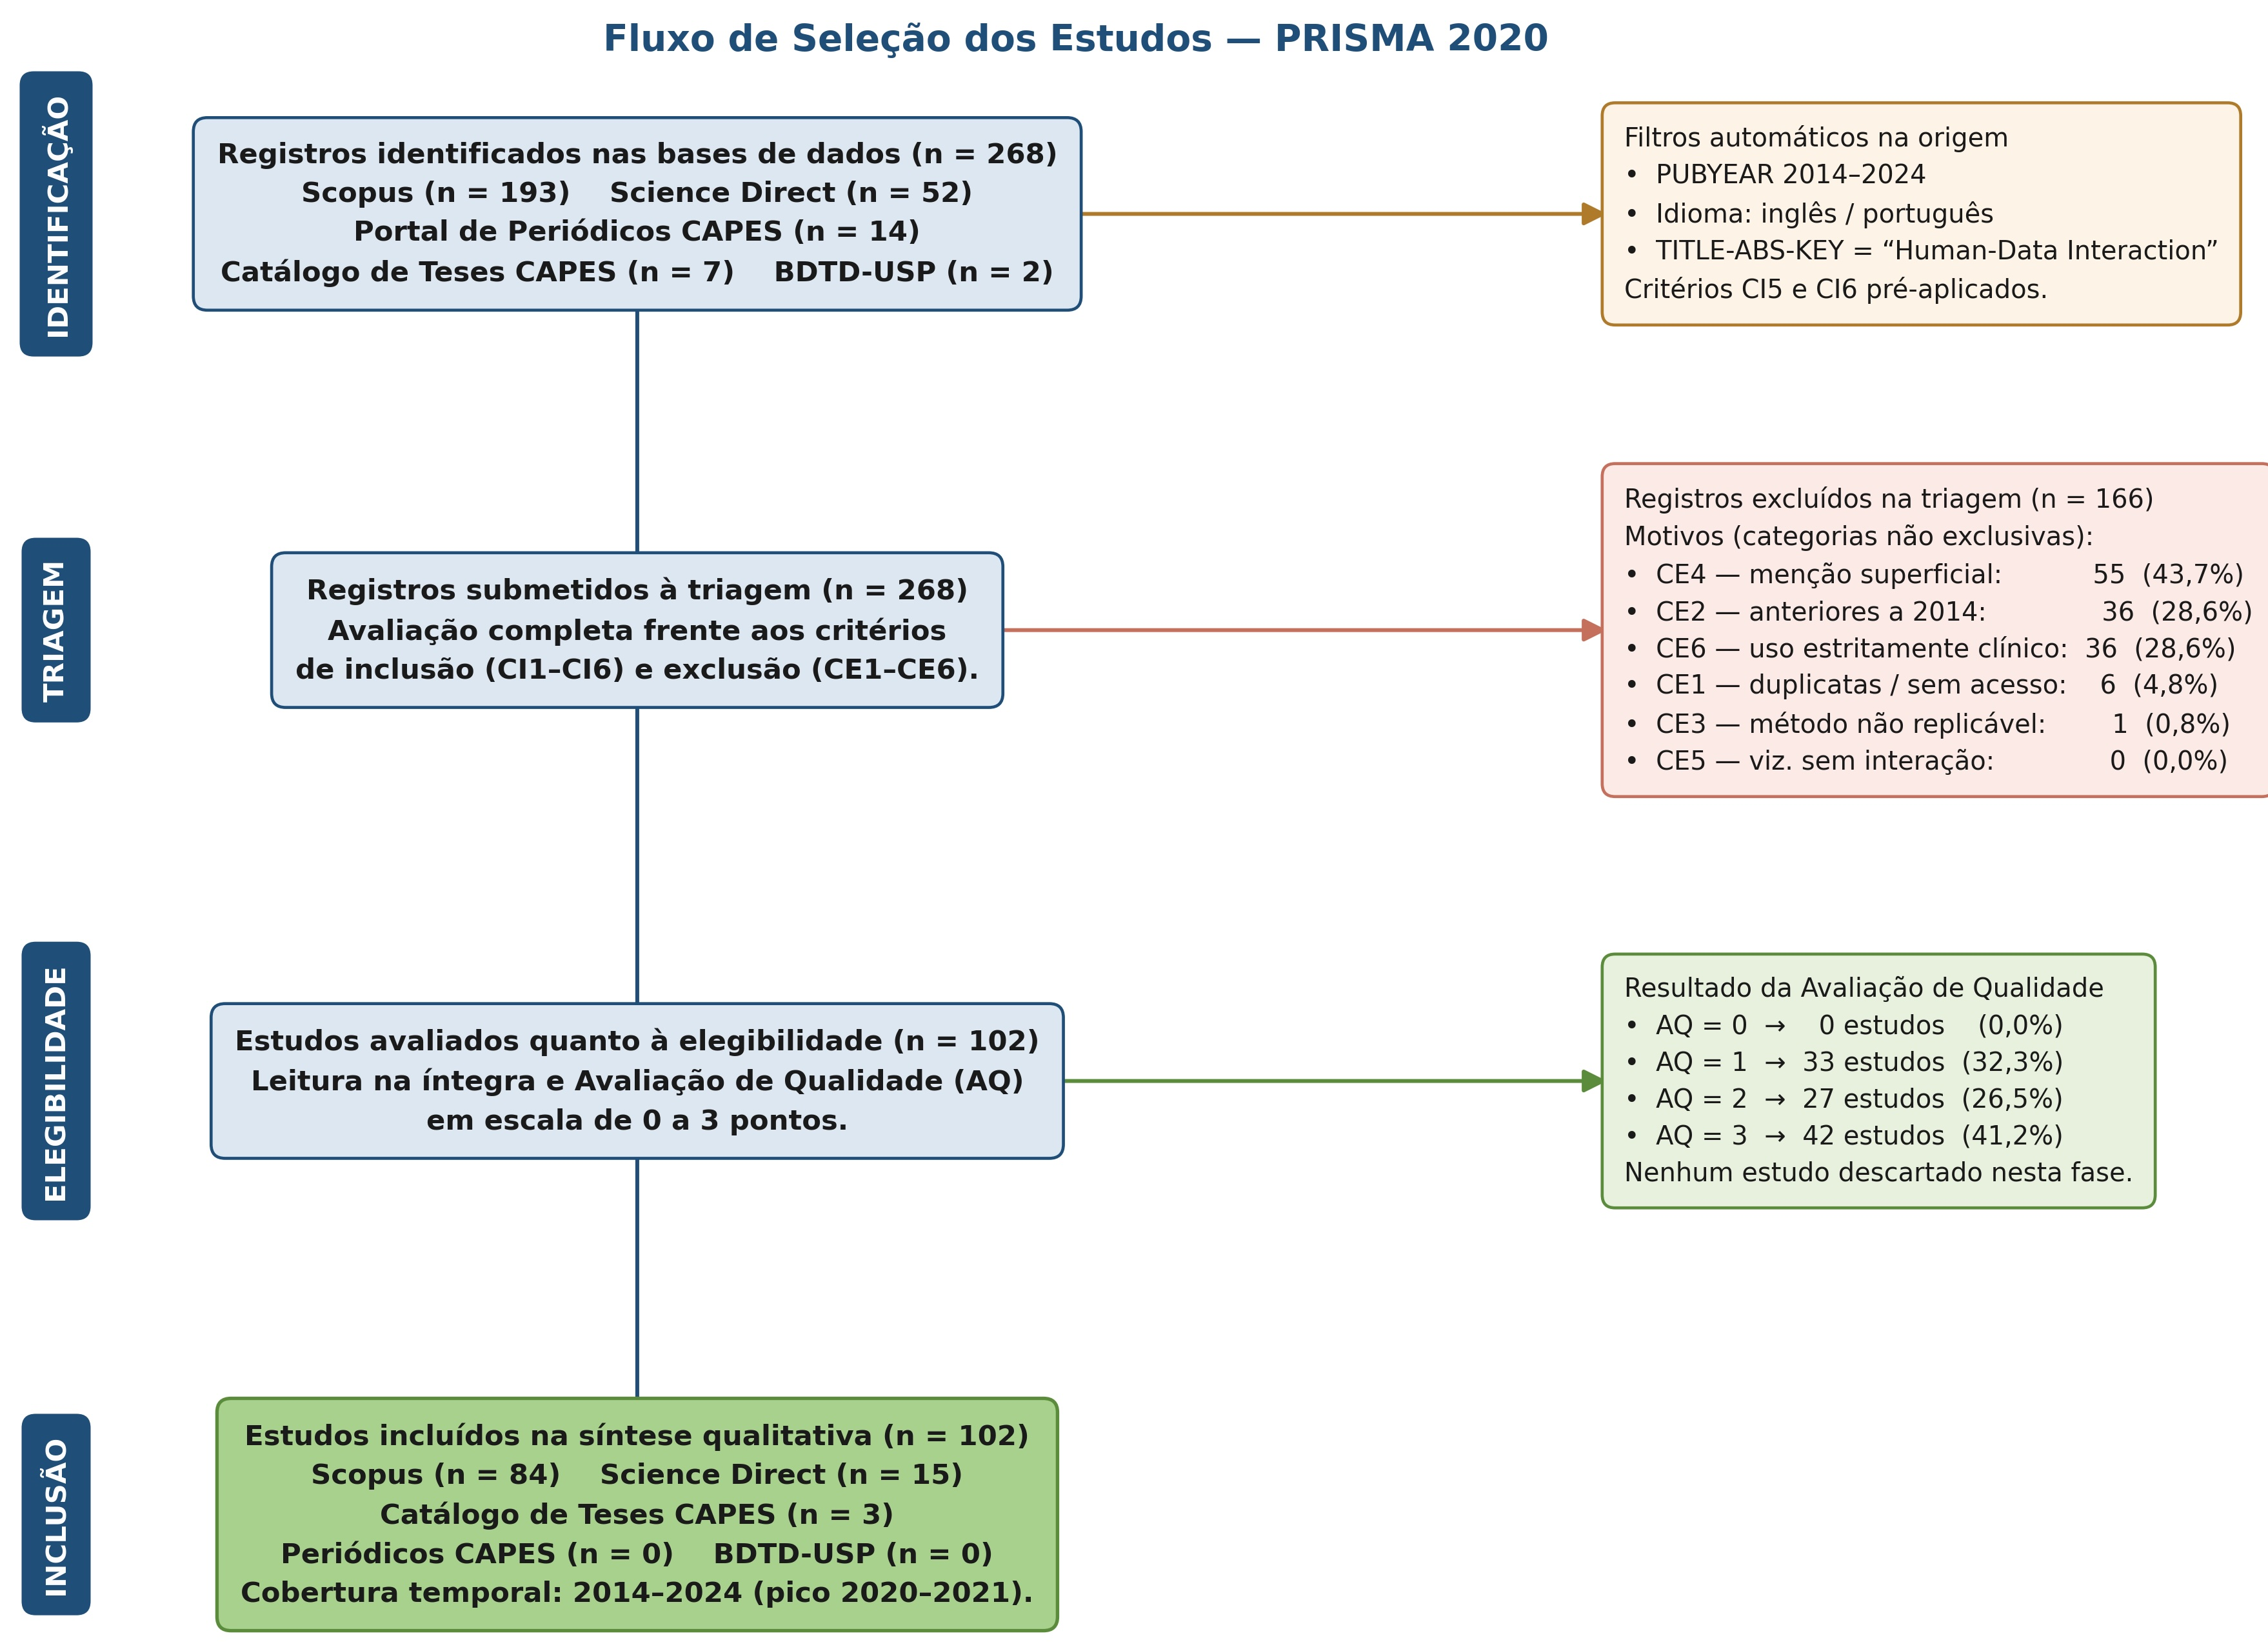
\includegraphics[width=0.9\linewidth]{Imagens/prisma_flow_v4.jpg}
    \caption{Fluxo de seleção dos estudos seguindo o protocolo PRISMA 2020 \hl{(descrição textual alternativa incluída para acessibilidade)}}
    \label{fig:prisma_flow}
\end{figure}

\subsection{Fontes de dados}

    Para a revisão sistemática, esta pesquisa utilizou fontes diversificadas que incluem bases internacionais e nacionais de relevância acadêmica. A \emph{Scopus\footnote{https://www.scopus.com}} foi selecionada como fonte principal devido ao seu escopo multidisciplinar, essencial para mapear a interseção entre tecnologia e o contexto urbano\hl{, e por indexar de forma agregada o conteúdo de editoras como Elsevier, ACM e IEEE, permitindo a padronização da extração de metadados via \textit{TITLE-ABS-KEY} sem exigir a repetição da busca em múltiplas plataformas nativas. Ainda assim, reconhece-se que essa escolha pode ter deixado de fora trabalhos indexados apenas em bases nativas como a ACM Digital Library e a IEEE Xplore, ou em repositórios brasileiros de acesso aberto como a SOL (Sociedade Brasileira de Computação Open Library), limitação retomada na Seção~}\ref{sec:ameacas}\hl{.}

    Adicionalmente, foram consultadas bases especializadas como o \emph{Science Direct\footnote{https://www.sciencedirect.com}} para acesso a publicações técnicas\hl{, dado seu peso editorial na literatura de urbanismo e sistemas ciberfísicos}, e o \emph{Portal de Periódicos CAPES\footnote{https://www.periodicos.capes.gov.br}} para a inclusão de produção científica nacional. Para abranger pesquisas acadêmicas brasileiras relevantes\hl{, incluindo teses e dissertações não necessariamente publicadas em periódicos indexados pela Scopus}, foram utilizados os \emph{Repositórios de Teses da USP\footnote{https://www.teses.usp.br}} e da \emph{CAPES\footnote{https://catalogodeteses.capes.gov.br}}.
    
    %Para a revisão sistemática, esta pesquisa utilizou fontes diversificadas que incluem bases internacionais e nacionais de relevância acadêmica reconhecida. A \emph{Scopus\footnote{https://www.scopus.com}} foi selecionada como fonte principal por seu amplo escopo, indexando artigos de alto impacto de editoras como Elsevier, IEEE Xplore e ACM Digital Library, além de oferecer cobertura de periódicos internacionais.

   %Adicionalmente, foram consultadas bases especializadas como o \emph{Science Direct\footnote{https://www.sciencedirect.com}} para acesso a publicações técnicas, e o \emph{Portal de Periódicos CAPES\footnote{https://www.periodicos.capes.gov.br}} para a inclusão de produção científica nacional. Para abranger pesquisas acadêmicas brasileiras relevantes, foram utilizados os \emph{Repositórios de Teses da USP\footnote{https://www.teses.usp.br}} e da \emph{CAPES\footnote{https://catalogodeteses.capes.gov.br}}.

\subsection{Período de Publicação}

   \hl{O período selecionado compreende os anos de 2014 a 2024, intervalo que acompanha a emergência da IHD como campo de estudo distinto. O marco inicial remete ao surgimento do termo na literatura acadêmica, impulsionado por trabalhos fundacionais} \hlcite{mortier2015humandatainteractionhumanface,Hornung2015}\hl{, que estabeleceram as bases da relação entre humanos e dados pessoais. Esta década permite rastrear desde a fundamentação teórica inicial até os estudos recentes que dialogam com as regulamentações globais de proteção de dados, como o Regulamento Geral de Proteção de Dados (GDPR)} \cite{gdpr2016}\hl{, refletindo os desafios contemporâneos da IHD no urbanismo de plataforma} \hlcite{Belizario2023Interacao,chalhoub2024useful,coleti2024grandihc}.

\subsection{Questões de Pesquisa}

 Esta revisão sistemática foi estruturada a partir de um conjunto de questões, elaboradas para mapear o estado da arte da Interação Humano-Dados (IHD) e identificar os desafios emergentes na área. As questões foram divididas em principais e secundárias:

\textbf{Questões Principais (QP):}
\begin{itemize}
\item \textbf{QP1} - Como a literatura sobre Interação Humano-Dados (IHD) evoluiu em conceito e prática na última década (2014-2024)?
\item \textbf{QP2} - Quais são as principais diferenças entre as abordagens teóricas e as implementações práticas relatadas na literatura nesse período?
\item \textbf{QP3} - Quais lacunas na pesquisa atual são recorrentemente citadas nos estudos?
\item \textbf{QP4} - \hl{Antes da emergência da IHD, tomando como marco divisor o trabalho fundacional de} \hlcite{mortier2015humandatainteractionhumanface} \hl{em 2015, conforme detalhado na Seção~}\ref{sec:referencial}\hl{,} quais abordagens facilitavam o entendimento sobre a gestão de dados em aplicações?
\item \textbf{QP5} - Qual é a importância da aplicação da IHD no contexto de \textit{Smart Cities}?
\end{itemize}

\textbf{Questões Secundárias (QPS):}
\begin{itemize}
\item \textbf{QPS1} - Quais métodos de avaliação (ex.: testes de usabilidade, \textit{eye-tracking}) são usados para medir a eficácia da IHD?
\item \textbf{QPS2} - Quais elementos de sistemas IHD ajudam usuários inexperientes digitalmente a compreender melhor os dados?
\item \textbf{QPS3} - Os estudos de caso analisados testaram algum \textit{framework} utilizando IHD?
\item \textbf{QPS4} - De que forma fatores étnico-culturais podem influenciar a aplicação da IHD?
\end{itemize}

Para fundamentar a busca e a seleção dos estudos destinados a responder a essas questões, o escopo da revisão foi delimitado utilizando uma adaptação da estrutura PICOC---do inglês Population, Intervention, Control, Outcomes, and Context (População, Intervenção, Controle, Resultados e Contexto/Aplicação):

\begin{itemize}
\item \textbf{População:} Trabalhos acadêmicos da área de IHD e pesquisas que demonstrem aplicações concretas dos seus princípios em diversos contextos.
\item \textbf{Intervenção:} Delimitação do escopo conceitual da IHD, mapeamento dos princípios teóricos fundamentais, metodologias de mensuração aplicáveis e identificação de lacunas.
\item \textbf{Controle:} Seleção sistemática priorizando trabalhos que proponham (re)formulações de princípios de IHD, apresentem aplicações práticas ou discutam métodos de avaliação.
\item \textbf{Resultados:} Sistematização do conhecimento sobre métodos e técnicas empregados e o mapeamento das lacunas frequentes na literatura.
\item \textbf{Aplicação:} Pesquisadores de IHD e IHC, além de profissionais da indústria que buscam compreender a aplicação e mensuração desses princípios na prática.
\end{itemize}

\subsection{Estratégia de Busca e Elegibilidade}
\label{estrategiaDeBusca}

    A estratégia de identificação dos estudos integrou parâmetros temáticos e cronológicos. Estabeleceu-se uma \textit{string} de busca base focada no termo ``Human-Data Interaction'', configurada inicialmente para a base Scopus---incidindo sobre título, resumo e palavras-chave (\textit{TITLE-ABS-KEY}). Esta equação principal foi adaptada à sintaxe específica e às regras de indexação de cada uma das outras plataformas \hl{, substituindo, por exemplo, o operador} \textit{TITLE-ABS-KEY} \hl{da Scopus pelos campos equivalentes de título/resumo/palavras-chave da ScienceDirect e do Portal de Periódicos CAPES, e ajustando os operadores booleanos e de truncamento} \hl{(\textit{wildcards})} \hl{conforme a sintaxe de cada} \hl{base}. \hl{Com vistas à reprodutibilidade, frente aos} limites de formatação do artigo, as \textit{strings} exatas utilizadas em todas as bases (incluindo parâmetros de indexação e recortes temporais) foram documentadas e disponibilizadas integralmente em um \emph{repositório suplementar}\footnote{https://anonymous.4open.science/r/sbc-rs-4046/Listas/Lista\%20de\%20Strings.txt}. O limite temporal da última década (2014--2024) foi parametrizado diretamente nos filtros de todas as bases, \hl{brangendo desde os marcos conceituais pioneiros da área (Seção}~\ref{sec:referencial}) \hl{até os desenvolvimentos mais recentes}.

    Foram elegíveis contribuições teóricas (\textit{frameworks} e princípios), artigos metodológicos sobre mensuração de usabilidade, estudos de caso em soluções urbanas e revisões sistemáticas correlatas. Quanto ao idioma, embora sem restrições formais iniciais, priorizaram-se publicações em inglês e português, escolha justificada pela predominância do inglês na literatura científica global e pela relevância do português para o contexto de aplicação urbano brasileiro que motiva esta pesquisa.
    
%A estratégia de identificação dos estudos integrou parâmetros temáticos e cronológicos. Estabeleceu-se uma \textit{string} de busca base focada no termo ``Human-Data Interaction'', configurada inicialmente para a base Scopus—incidindo sobre título, resumo e palavras-chave (\textit{TITLE-ABS-KEY}). Esta equação principal foi adaptada à sintaxe específica e às regras de indexação de cada uma das outras plataformas, sendo as \textit{strings} exatas de cada repositório detalhadas no Apêndice A (ou Tabela X). O limite temporal da última década (2014-2024) foi parametrizado diretamente nos filtros de todas as bases, abrangendo desde os marcos conceituais pioneiros até os desenvolvimentos mais recentes da área.
%A estratégia de identificação dos estudos integrou parâmetros temáticos e cronológicos. Estabeleceu-se uma \textit{string} de busca base focada no termo ``Human-Data Interaction'', configurada inicialmente para a base Scopus—incidindo sobre título, resumo e palavras-chave (\textit{TITLE-ABS-KEY}). Esta equação principal foi adaptada à sintaxe específica e às regras de indexação de cada uma das outras plataformas. O limite temporal da última década (2014-2024) foi parametrizado diretamente nos filtros de todas as bases, abrangendo desde os marcos conceituais pioneiros até os desenvolvimentos mais recentes da área\footnote{https://anonymous.4open.science/r/sbc-rs-4046/Listas/Scopus\_Lista\%20de\%20artigos.txt}\footnote{https://anonymous.4open.science/r/sbc-rs-4046/Listas/Sicence\%20Direct\_Lista\%20de\%20artigos.txt}\footnote{https://anonymous.4open.science/r/sbc-rs-4046/Listas/Periódicos\%20Capes\_Lista\%20de\%20artigos.txt}\footnote{https://anonymous.4open.science/r/sbc-rs-4046/Listas/Teses\%20USP\_Lista\%20de\%20Teses.txt}\footnote{https://anonymous.4open.science/r/sbc-rs-4046/Listas/Teses\%20Capes\_Lista\%20de\%20teses.txt}.

%Foram elegíveis contribuições teóricas (\textit{frameworks} e princípios), artigos metodológicos sobre mensuração de usabilidade, estudos de caso em soluções urbanas e revisões sistemáticas correlatas. Quanto ao idioma, embora sem restrições formais iniciais, priorizaram-se publicações em inglês e português, escolha justificada pela predominância do inglês na literatura científica global e pela relevância do português para o contexto de aplicação urbano brasileiro que motiva esta pesquisa.

\subsection{Critérios de Seleção e Avaliação de Qualidade}

  Para estruturar a seleção dos estudos e sistematizar o conhecimento sobre o estado da arte em IHD no contexto urbano, foram estabelecidos critérios de inclusão (CI) e exclusão (CE), documentados nas \emph{tabelas resultantes da execução da RSL}\footnote{https://anonymous.4open.science/r/sbc-rs-4046/Tabelas/}. Esses parâmetros, detalhados na Tabela~\ref{tab:criterios}, \hl{buscam equilibrar } abrangência teórica e especificidade prática, priorizando trabalhos replicáveis, disponíveis na íntegra e alinhados ao recorte temporal (2014–2024).

\begin{table}[H]
\centering
\caption{Critérios de Inclusão (CI) e Exclusão (CE)}
\label{tab:criterios}
\small
\begin{tabular}{p{0.12\linewidth} p{0.8\linewidth}}
\hline
\textbf{Código} & \textbf{Descrição do Critério} \\ 
\hline
\multicolumn{2}{c}{\textbf{Critérios de Inclusão (CI)}} \\ 
\hline
\textbf{CI1} & Trabalhos que definam, aprimorem ou proponham \textit{frameworks} para princípios teóricos de IHD. \\ 
\textbf{CI2} & Pesquisas que desenvolvam ou validem métricas de avaliação em IHD. \\ 
\textbf{CI3} & Artigos com resultados empíricos ou modelos teóricos validados (ex.: estudos de caso, experimentos). \\ 
\textbf{CI4} & Revisões sistemáticas anteriores que ofereçam contribuições originais à teoria. \\ 
\textbf{CI5} & Publicações revisadas por pares (conferências indexadas ou periódicos). \\
\textbf{CI6} & Trabalhos publicados entre 2014 e 2024. \\
\hline
\multicolumn{2}{c}{\textbf{Critérios de Exclusão (CE)}} \\
\hline
\textbf{CE1} & Artigos duplicados, indisponíveis na íntegra ou que exijam pagamento para acesso. \\
\textbf{CE2} & Trabalhos publicados antes de 2014. \\
\textbf{CE3} & Metodologia não replicável ou sem descrição clara dos métodos. \\
\textbf{CE4} & Menção superficial à IHD, sem focar em princípios, \textit{frameworks} ou métricas. \\
\textbf{CE5} & Estudos sobre visualização de dados sem componente de interação humana. \\
\textbf{CE6} & Uso do termo ``IHD'' em contextos não relacionados ou voltados estritamente a procedimentos clínicos sem dimensão de interação cidadã/usuária. \\
\hline
\end{tabular}
\end{table}

Após a filtragem por CI e CE, os estudos elegíveis foram submetidos a uma Avaliação de Qualidade (AQ), documentada nas \emph{tabelas da RSL}\footnote{https://anonymous.4open.science/r/sbc-rs-4046/Tabelas/}. Esta etapa avaliou a contribuição de cada artigo para as questões de pesquisa, utilizando um sistema de pontuação \hl{baseado na abrangência com que cada estudo cobre os temas principais da revisão, definidos pelas questões de pesquisa (QP e QPS) --- que contemplam os princípios de IHD (legibilidade, agência e negociabilidade), sua aplicação em contextos urbanos (\textit{Smart Cities}) e a gestão de dados do usuário ---, conforme a Tabela~}\ref{tab:qualidade}. Apenas artigos com \hl{maior pontuação} (2 ou 3 pontos) foram priorizados para análise integral e extração de dados.

\begin{table}[H]
\centering
\caption{Sistema de Pontuação para Avaliação de Qualidade (AQ)}
\label{tab:qualidade}
\small
\begin{tabular}{c p{0.75\linewidth}}
\hline
\textbf{Pontos} & \textbf{Nível de Contribuição do Artigo} \\ 
\hline
\textbf{0} & Sem contribuição metodológica ou teórica relevante para as Questões de Pesquisa. \\ 
\hline
\textbf{1} & Aborda apenas um dos temas principais da pesquisa de forma isolada. \\ 
\hline
\textbf{2} & Relaciona adequadamente dois dos temas principais da pesquisa. \\ 
\hline
\textbf{3} & Integra de forma robusta três ou mais temas principais da pesquisa. \\ 
\hline
\end{tabular}
\end{table}

\subsection{Condução das Buscas e Triagem dos Estudos}

As buscas foram executadas nas cinco bases de dados selecionadas, adaptando-se a \textit{string} principal (``Human-Data Interaction'') e o recorte temporal (2014 a 2024) às especificidades sintáticas de cada \hl{base} (ex.: uso do comando \texttt{PUBYEAR} na Scopus). A triagem por título e resumo e a aplicação dos critérios de inclusão/exclusão foram conduzidas \hl{pela autora principal e, posteriormente, revisadas e validadas pelo orientador, também autor deste trabalho, o que introduziu uma verificação independente das decisões de inclusão}. Para reduzir a \hl{subjetividade da triagem inicial}, a decisão de inclusão foi orientada pela \hl{pontuação sistemática} dos artigos segundo a matriz de Avaliação de Qualidade (Tabela~\ref{tab:qualidade}), cujos registros individuais por artigo estão disponíveis no repositório suplementar\footnote{https://anonymous.4open.science/r/sbc-rs-4046/Tabelas/}, permitindo a auditoria externa dos critérios aplicados a cada estudo. Ainda assim, a ausência de \hl{uma dupla triagem independente e cega constitui uma limitação reconhecida do processo de seleção}, discutida na Seção~\ref{sec:ameacas}.

O levantamento bruto inicial retornou um total de \textbf{268 documentos}. A aplicação dos critérios de elegibilidade resultou em um \textit{corpus} final de \textbf{102 trabalhos} aprovados para a etapa de extração de dados e leitura na íntegra. A Tabela \ref{tab:funil_selecao} consolida o funil de seleção detalhado por repositório.

\begin{table}[H]
\centering
\caption{Consolidação do Funil de Seleção de Estudos por Base de Dados}
\label{tab:funil_selecao}
\small
\begin{tabular}{p{0.40\linewidth} c c c}
\hline
\textbf{Base de Dados} & \textbf{Retorno Inicial} & \textbf{Excluídos} & \textbf{Incluídos} \\ \hline
Scopus & 193 & 109 & 84 \\
Science Direct & 52 & 37 & 15 \\
Portal de Periódicos CAPES & 14 & 14 & 0 \\
Catálogo de Teses CAPES & 7 & 4 & 3 \\
BDTD-USP & 2 & 2 & 0 \\ \hline
\textbf{Total} & \textbf{268} & \textbf{166} & \textbf{102} \\ \hline
\end{tabular}
\end{table}
\vspace{-0.1 cm} 

\hl{A análise das 166 exclusões mostrou predominância de trabalhos fora do escopo conceitual da IHD.} As remoções concentraram-se em abordagens superficiais da IHD (\textbf{CE4}) ou no uso do acrônimo em contextos puramente médicos e de \textit{hardware} de baixo nível (\textbf{CE6}). Nas bases agregadoras (CAPES e BDTD-USP), o índice de exclusão total deveu-se estritamente à sobreposição de duplicatas (\textbf{CE1}) já retidas na busca primária (Scopus). \hl{Esse comportamento indica que a estratégia atingiu boa cobertura}, resultando em um \textit{corpus} final de 102 artigos \hl{relevantes para as questões de pesquisa.}

\hl{Na Avaliação de Qualidade (AQ), em escala de 0 a 3 para avaliar a cobertura dos temas de interesse da revisão---como os princípios de IHD, as cidades inteligentes, a governança de dados e as questões sociotécnicas---, nenhum trabalho obteve pontuação nula, o que é coerente com o critério de seleção adotado, que priorizou estudos alinhados a esses temas.}

A Tabela~\ref{tab:resumo_qualidade} sintetiza a \hl{distribuição das pontuações de qualidade do acervo}. A maior parcela alcançou a \hl{pontuação} máxima \emph{3} (\textbf{42} estudos, 41,2\%), \hl{integrando três ou mais eixos temáticos}. Os demais distribuíram-se entre a \hl{pontuação} \emph{2} (\textbf{27} artigos, 26,5\%), \hl{que relaciona dois eixos}, e a \hl{pontuação} \emph{1} (\textbf{33} artigos, 32,3\%), \hl{restrita a um único eixo}. \hl{A concentração de estudos nos níveis 2 e 3 (67,7\% do acervo) indica que a maior parte das publicações retidas articula mais de um dos eixos temáticos de interesse.}

\begin{table}[H]
\centering
\caption{Resultados da Avaliação de Qualidade (AQ)}
\label{tab:resumo_qualidade}
\small
\begin{tabular}{p{0.55\linewidth} c c}
\hline
\textbf{Pontuação (Nível de Contribuição)} & \textbf{Quantidade} & \textbf{Percentual} \\
\hline
(0) Sem contribuição teórica ou metodológica relevante & 0 & 0,0\% \\
(1) Aborda apenas um tema principal isoladamente & 33 & 32,3\% \\
(2) \hl{Relaciona dois temas principais} & 27 & 26,5\% \\
(3) \hl{Integra três ou mais temas principais}  & 42 & 41,2\% \\
\hline
\textbf{Total} & \textbf{102} & \textbf{100,0\%} \\
\hline
\end{tabular}
\end{table}

Em síntese, com o \textit{corpus} \hl{definido}, a pesquisa avança \hl{para a análise destas publicaçõe}s, visando responder às Questões de Pesquisa (QPs) e \hl{mapear} o estado da arte e as lacunas da governança de dados em sistemas sociotécnicos urbanos.

\subsection{Análise da Triagem e Perfil da Literatura}

% A triagem inicial avaliou \textbf{268} documentos, resultando na inclusão de \textbf{102} trabalhos. Essa taxa de retenção de 38\% reflete a aplicação de um filtro rigoroso para consolidar um \textit{corpus} robusto. Majoritariamente, os estudos selecionados atenderam a múltiplos critérios simultâneos, articulando \textit{frameworks} práticos (\textbf{CI1}), validação por revisão por pares (\textbf{CI5}), resultados empíricos (\textbf{CI3}) e o desenvolvimento de métricas de avaliação (\textbf{CI2}). Essa convergência demonstra que a literatura em IHD já transita da fundamentação conceitual para aplicações validadas, fornecendo subsídios vitais para esta análise.

% O alinhamento ao recorte temporal da última década (2014-2024) (\textbf{CI6}) reflete a emergência recente do tema. A atualidade do acervo garante que os debates sobre legibilidade e agência estejam alinhados aos desafios contemporâneos de privacidade e governança de dados.

% Em contrapartida, as \textbf{166} exclusões seguiram padrões claros: concentraram-se em abordagens superficiais da IHD (\textbf{CE4}) ou no uso do acrônimo em contextos estritamente médicos e desvinculados da interação humana (\textbf{CE6}). A remoção rigorosa de duplicatas (\textbf{CE1}) e de documentos com barreiras de acesso completou o funil. Essa limpeza metodológica contribui para um referencial teórico centrado no usuário e no desenvolvimento de aplicações urbanas.

A triagem inicial avaliou \textbf{268} documentos, resultando na inclusão de \textbf{102} trabalhos. \hl{Essa taxa de retenção de 38\% resultou da aplicação dos critérios de elegibilidade}. \hl{Parte expressiva} dos estudos selecionados atendeu a múltiplos critérios \hl{de inclusão}, articulando \textit{frameworks} práticos (\textbf{CI1}), validação por revisão por pares (\textbf{CI5}), resultados empíricos (\textbf{CI3}) e o desenvolvimento de métricas de avaliação (\textbf{CI2}). \hl{Essa convergência sugere que a literatura em IHD tem transitado da fundamentação conceitual para aplicações validadas, fornecendo subsídios relevantes para esta análise.}

O \hl{recorte temporal adotado, referente à última década (2014--2024) (\textbf{CI6}), acompanha} a emergência recente do tema. A análise da distribuição temporal do \textit{corpus}, sintetizada na Figura~\ref{fig:distribuicao_ano_fonte}, evidencia três fases distintas na \hl{trajetória} da IHD aplicada a contextos urbanos. Entre 2014 e 2019, observa-se produção incipiente, com 24 trabalhos publicados ao longo de seis anos (23,5\% do \textit{corpus}). O biênio 2020-2021 concentra 43 artigos (42,2\%), pico que coincide temporalmente com a aceleração das pesquisas em dataficação urbana no contexto pandêmico e com a sedimentação de marcos regulatórios como \hl{o Regulamento Geral de Proteção de Dados (GDPR), em vigor desde 2018}. Em 2022-2024, o volume de publicações estabiliza-se entre 9 e 13 artigos por ano (35 trabalhos, 34,3\%), padrão sugestivo de \hl{estabilização da produção do campo}. A predominância da Scopus em todos os anos (cerca de 83\% do \textit{corpus}) corrobora a opção metodológica descrita na Seção~\ref{estrategiaDeBusca}, enquanto a contribuição pontual das Teses CAPES (2019, 2023 e 2024) sinaliza a entrada gradual da produção brasileira no debate.

\begin{figure}[H]
    \centering
    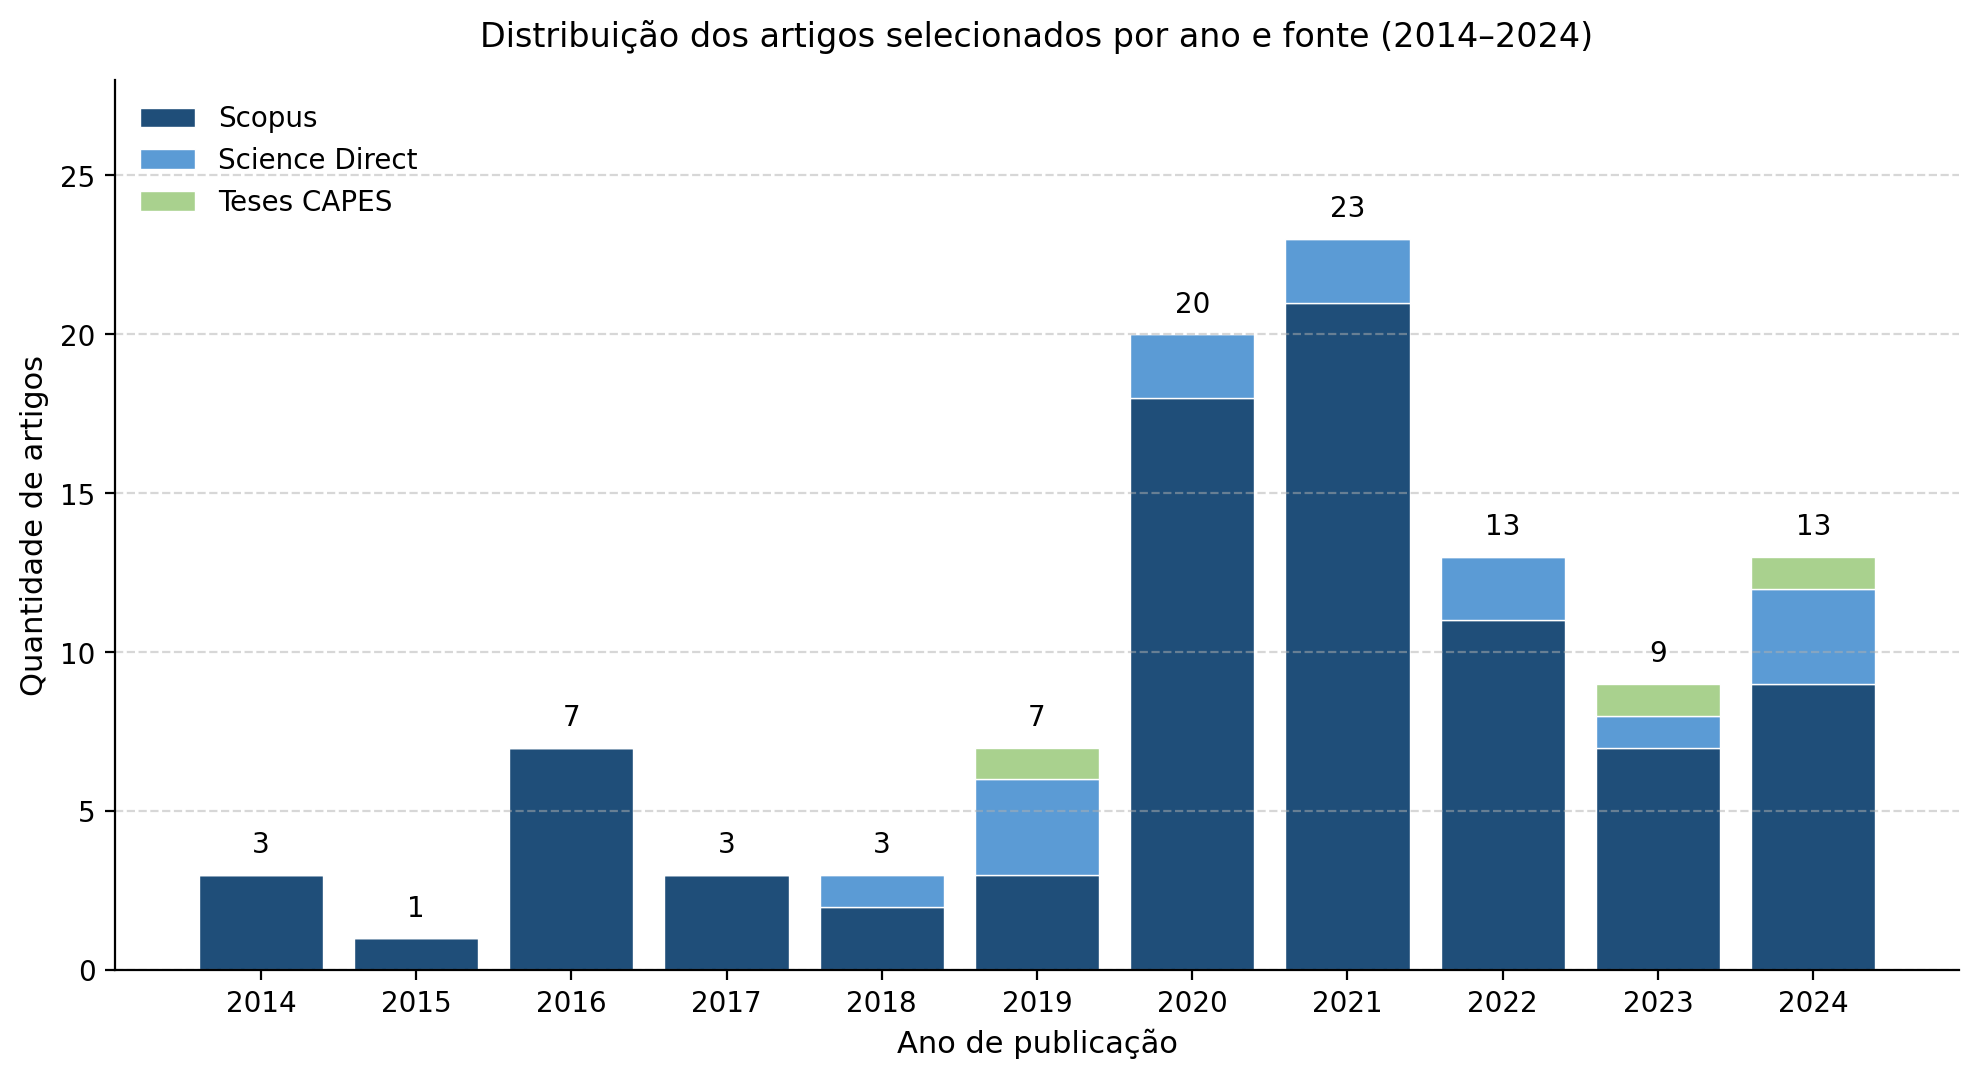
\includegraphics[width=0.95\linewidth]{Imagens/distribuicao_artigos_por_ano_empilhado.png}
    \caption{Distribuição dos 102 artigos do \textit{corpus} por ano e fonte (2014--2024). \hl{(descrição textual alternativa incluída para acessibilidade)}}
    \label{fig:distribuicao_ano_fonte}
\end{figure}

Em contrapartida, as \textbf{166} exclusões \hl{concentraram-se em poucos critérios}: abordagens superficiais da IHD (\textbf{CE4}) ou \hl{o} uso do acrônimo em contextos estritamente médicos e desvinculados da interação humana (\textbf{CE6}). A remoção de duplicatas (\textbf{CE1}) e de documentos com barreiras de acesso completou o funil. \hl{Esse processo de exclusão manteve o \textit{corpus} alinhado ao escopo conceitual da IHD e ao foco em aplicações urbanas.}

\subsection{Avaliação de Qualidade dos Estudos}

    Após a etapa de triagem, os \textbf{102} trabalhos do \textit{corpus} final foram submetidos à matriz de avaliação de qualidade, \hl{visando avaliar a cobertura de suas contribuições em relação aos temas de interesse da revisão}. A inexistência de artigos com pontuação nula \hl{é coerente com o critério de seleção adotado, indicando que todas as publicações retidas cobrem ao menos um desses temas.}

    A distribuição das avaliações \hl{reparte-se por três níveis de cobertura temática}. No estrato superior da matriz, \textbf{42} artigos (41,2\%) alcançaram a pontuação máxima (\textbf{3}). Caracterizados por abordar três ou mais temas de forma integrada, estes estudos \hl{articulam múltiplos temas de interesse, como} princípios teóricos, métricas e evidências empíricas, \hl{servindo de base} para as discussões transversais desta revisão. \hl{Um} grupo de \textbf{27} artigos obteve a pontuação \textbf{2} (26,5\%), \hl{relacionando a formulação teórica da IHD e sua implementação prática}. Por fim, \textbf{33} trabalhos (32,3\%) receberam a pontuação \textbf{1}\hl{: abordam um único eixo temático, com foco em facetas específicas da interação, como transparência e letramento de dados}.

    Em suma, a transição da triagem para a avaliação \hl{resultou em um referencial bibliográfico que abrange diferentes níveis de cobertura temática}. \hl{A composição do \textit{corpus} --- com estudos que integram três ou mais temas (nível 3), que relacionam dois (nível 2) e que abordam um único eixo (nível 1) --- fornece subsídios para a análise do estado da arte.}

\section{Resultados e Discussão}
\label{sec:resultados}

A análise \hl{dos} 102 trabalhos incluídos na Revisão Sistemática permitiu mapear \hl{a evolução histórica e estrutural} da Interação Humano-Dados (IHD)\hl{.} \hl{A documentação completa encontra-se nas} \emph{tabelas da RSL}\footnote{https://anonymous.4open.science/r/sbc-rs-4046/Tabelas/}. Com base na extração sistemática de evidências qualitativas, esta seção apresenta a síntese crítica da literatura, organizada em eixos temáticos que respondem de forma transversal e detalhada às Questões de Pesquisa (QPs e QPSs) delineadas no protocolo metodológico.

\subsection{A Evolução da Gestão de Dados e o Descompasso Sociotécnico (QP1, QP4)}

    Antes da \hl{emergência} da IHD, a literatura evidencia que as abordagens para a gestão de dados fundamentavam-se em um paradigma \hl{predominantemente} tecnocrático e centrado na máquina. O foco primário das pesquisas \hl{concentrava-se} no aprimoramento de tecnologias de Tomada de Decisão Apoiada por Dados (\textit{Data-Supported Decision Making}), priorizando a eficiência do processamento bruto e a segurança algorítmica corporativa em detrimento da carga cognitiva do usuário \cite{calvetti2024human, Locoro2020}. Nesse contexto, o desenvolvimento de \textit{software} operava majoritariamente confinado às camadas física, empírica e sintática da Escada Semiótica (modelo teórico que categoriza os sistemas de informação desde a infraestrutura técnica até o seu impacto no mundo real) \hlcite{Hornung2015}, \hl{negligenciando} as dimensões sociais, semânticas e pragmáticas que caracterizam a onipresença informacional na vida cotidiana \cite{Strey2019Human}.

    Nesse período pré-IHD, a proteção informacional ancorava-se \hl{no} modelo burocrático de ``Aviso e Escolha'' (\textit{Notice and Choice}). \hl{Herdado de contextos regulatórios anteriores}, esse mecanismo fundamentava-se na apresentação de termos \hl{extensos} para a obtenção de um consentimento binário, transferindo a responsabilidade legal ao usuário {\hlcite{Jones2017}. Aliada a isso, havia a imposição de Contratos de Licença de Usuário Final (\textit{End-User License Agreements}---EULAs) \hl{que operavam} como instrumentos de adesão unilaterais e inegociáveis (\textit{take-it-or-leave-it}). Redigidos em \hl{linguagem técnico-jurídica de difícil compreensão}, tais contratos condicionavam o acesso ao serviço à aceitação \hl{de} toda a extração de dados {\hlcite{Hutton2017}.

    A governança da época era regida por marcos regulatórios iniciais, como a Diretiva 95/46/CE,\footnote{Disponível em: https://eur-lex.europa.eu/legal-content/PT/TXT/?uri=CELEX:31995L0046. Acesso em: 20 maio 2026.} antecessora do Regulamento Geral \hl{de} Proteção de Dados (\textit{General Data Protection Regulation}---GDPR)\footnote{Disponível em: https://\hl{eur-lex}.europa.eu/legal-content/PT/TXT/?uri=CELEX:32016R0679. Acesso em: 20 maio 2026.}, que regulava o fluxo em uma arquitetura de internet ainda incipiente---e por conceitos estritos de Direito de Propriedade. Essa visão tratava o dado digital, que é altamente replicável e relacional, como um objeto físico isolado, \hl{enquadramento que a literatura aponta como inadequado} \cite{malgieri2019automated, janecek2018ownership}. \hl{Essa abordagem} baseada em \textit{walled gardens} (metáfora para ecossistemas proprietários onde plataformas monopolizam a custódia dos dados e restringem a interoperabilidade) \hlcite{Turkay2021, Xiao2021} \hl{revelou limitações significativas, associadas à racionalidade limitada do ser humano} frente à assimetria de poder e à proteção legal garantida às corporações, \hl{bem como à} sobrecarga cognitiva gerada por termos de uso \hl{extensos} \cite{malgieri2020vulnerable, DOWTHWAITE2024, chalhoub2024useful}.
    
    Nesse cenário, a Interação Humano-Computador (IHC) clássica \hl{mostrou-se limitada para} lidar com as consequências éticas e os riscos sociopsicológicos do processamento de dados invisível e onipresente em rede \hlcite{Parviainen2016, Calvetti2021173}. \hl{Isso se deve ao fato de que} a área concentrava seus esforços na usabilidade de \textit{hardware} e em métricas de eficiência pontuais, como o tempo de execução de tarefas em telas bidimensionais. Tratava-se de um modelo voltado para ambientes onde o indivíduo interagia de forma \hl{deliberada} com uma interface visível, \hl{sem contemplar} a extração ubíqua de rastros digitais.

     A evolução do campo documentada na última década (2014-2024) sinaliza uma \hl{transição} epistemológica e metodológica. Historicamente, os primeiros estudos que tangenciavam a IHD, \hl{no início da década}, focavam predominantemente na análise técnica de conjuntos massivos de informações\hlcite{Parviainen2016, Meireles2016, Hornung2015}. \hl{No entanto, é a partir do trabalho fundacional de 2015} \cite{mortier2015humandatainteractionhumanface} \hl{que a IHD emerge como campo ético e conceitual autônomo}.

    Sob essa nova perspectiva, os dados deixam de ser concebidos como meras entradas passivas do sistema para se tornarem objetos de primeira classe (\textit{first-class objects}) \hlcite{Crabtree2016}. Isso significa que eles passam a atuar como entidades computacionais autônomas que detêm privilégios primários na arquitetura do \textit{software}, podendo ser manipulados, transferidos e auditados diretamente, sem subordinação a outras estruturas funcionais. Consequentemente, esses ativos sociotécnicos passam a exigir tratamento \hl{como material de design} \cite{seidelin2020foregrounding}, significando que a informação passa a ser tratada como um recurso plástico, moldável e intencionalmente configurado para mediar a experiência humana, e não como um subproduto inerte da programação. 

    A prática acadêmica e projetual transita, portanto, da criação de interfaces isoladas para a compreensão de ecossistemas complexos. Busca-se integrar o comportamento e as expectativas do indivíduo no ciclo de vida das infraestruturas urbanas, cenário em que o cidadão deixa de ser um espectador técnico e assume o papel de \hl{agente ativo, dotado de agência e autonomia} \cite{Sailaja2021Designing, bavaresco2019technological}.

    Apesar do potencial dessa virada conceitual, a revisão sistemática revela contrastes e fricções na transição da teoria para a prática implementada. No pilar da \textbf{legibilidade}, a literatura teórica avançou da mera exibição de painéis estáticos (\textit{dashboards}) para a promoção da construção ativa de sentido (\textit{data sensemaking}), estruturada em eixos de inspeção, engajamento e contextualização da informação \hlcite{Koesten2021}. Contudo, as implementações reais em ecossistemas digitais ainda \hl{apresentam} jargões técnicos \hl{de difícil compreensão} e fluxos de decisão não lineares \cite{Sailaja2021}.

    No pilar da \textbf{agência}, o conceito evoluiu da aceitação de modelos de consentimento binários para arquiteturas de prestação de contas (\textit{accountability}) \cite{janecek2018ownership}. Nesses novos paradigmas sociotécnicos, o cidadão não se limita a visualizar o que foi armazenado. Ele passa a dispor de mecanismos concretos para rastrear o fluxo informacional, auditar decisões algorítmicas e exigir justificativas claras sobre o processamento de suas informações, sendo promovido à figura de administrador (\textit{steward}) de seus próprios rastros digitais \cite{angelopoulos2021stewardship}. 

    Todavia, a revisão indica que projetistas e desenvolvedores novatos enfrentam barreiras na prática. Sem o suporte metodológico de diretrizes operacionais ou heurísticas validadas, torna-se complexo aplicar esses artefatos teóricos durante o desenvolvimento de \textit{software} \cite{Strey2019Human, Victorelli2020Human, chalhoub2024useful}. 

    Por fim, a \textbf{negociabilidade} expandiu-se das interações mediadas por telas para a governança difusa de dados passivos, como aqueles capturados ininterruptamente por sensores em espaços urbanos \hlcite{Locoro2020}---isto é, o gerenciamento ético de informações extraídas de forma invisível, ambiental e onipresente por infraestruturas de Internet das Coisas (IoT), frequentemente sem qualquer engajamento intencional ou consciência por parte do transeunte. Contudo, a efetivação dessa dimensão de negociabilidade na prática urbana depara-se com a fragmentação expressiva das ferramentas de controle e com a carência de padrões estruturais unificados, fatores que comprometem o estabelecimento de um diálogo simétrico, contínuo e participativo entre a população e os sistemas que a monitoram \hlcite{Chatzimichali2021160}.
        
    \subsection{Lacunas Estruturais, Desafios Cognitivos e Opacidade (QP2, QP3)}

    A análise do acervo selecionado revela que a IHD, embora conceitualmente estruturada, ainda enfrenta lacunas estruturais que dificultam sua implementação em larga escala \hlcite{Sailaja2021Designing, Strey2019Human}. Persiste a falta de um paradigma produtivo consolidado e a carência de um conjunto de heurísticas de \textit{design} validadas para orientar desenvolvedores em domínios específicos, com destaque para o contexto de geoprocessamento \hlcite{Capeleti2024Human}. Ademais, a literatura ainda \hl{apresenta ambiguidades na definição dos perfis e do usuário final das plataformas de dados urbanos} \hlcite{Belizario2023Interacao} e carece de especificações técnicas sobre o que torna um conjunto de dados abertos efetivamente reutilizável \hlcite{Koesten2020}.

    Uma lacuna \hl{frequentemente} negligenciada refere-se à sobrecarga cognitiva imposta aos usuários \cite{Locoro2020}. A literatura aponta um impacto sociopsicológico negativo decorrente da onipresença informacional, manifesto na \hl{fadiga cognitiva} e na ansiedade informacional \cite{cezar2023cognitive}. Esse estado ocorre quando o indivíduo experimenta \hl{estresse informacional} devido à percepção de perda de controle sobre a destinação e o uso de seus registros pessoais.

    Pesquisadores sublinham, por exemplo, a ausência de modelos mentais maduros para lidar com tecnologias emergentes, como a Identidade Autossoberana (\textit{Self-Sovereign Identity}---SSI). Esse paradigma de arquitetura digital descentralizada foi estruturado para permitir que o cidadão gerencie autonomamente suas próprias credenciais, sem depender de provedores centrais. No entanto, sua operação ainda se revela excessivamente complexa para o público leigo \cite{Lockwood2021, Lockwood2020AnAccessible}. Consequentemente, persiste uma escassez de estudos que cruzem a visão técnica dos especialistas em engenharia com a percepção de usabilidade e o modelo mental do cidadão comum \hlcite{Lockwood2020AnAccessible}.

   A integração ética com Inteligência Artificial e algoritmos corporativos emerge como outra área de vulnerabilidade significativa. Ferramentas automatizadas de \textit{Data-to-Text}, por exemplo, frequentemente falham por não capturarem o julgamento humano e as nuances pragmáticas do contexto informacional \hlcite{Haghighati2020}. Além disso, a legibilidade algorítmica esbarra recorrentemente no sigilo industrial e na opacidade das caixas-pretas corporativas, comprometendo o Direito à Explicação das decisões automatizadas que afetam a rotina do cidadão \cite{Barreto2018} \hlcite{DeAlmeida2019}.

    No âmbito das plataformas de gestão, a literatura evidencia a ineficácia prática dos atuais Serviços de Gestão de Dados Pessoais (PDMS)---repositórios onde o indivíduo deveria centralizar o controle de suas informações. A falha estrutural dessas plataformas revela a carência de soluções de \textit{design} que consigam conciliar a pressão comercial do extrativismo de dados com a real preservação da agência do usuário \hlcite{angelopoulos2021stewardship}.

    Por fim, a transposição empírica dos princípios da IHD para comunidades desfavorecidas constitui um desafio analítico ainda não superado. Estudos evidenciam a escassez de investigações empíricas sobre a inclusão de populações vulneráveis e demonstram como a \hl{dataficação} frequentemente exacerba as disparidades digitais pré-existentes \cite{hayes2024making, Locoro2020}. O equilíbrio entre a otimização de serviços em Cidades Inteligentes e a proteção da privacidade permanece classificado na literatura como um ``problema perverso'' (\textit{wicked problem})---um desafio de formulação interdependente, de natureza sistêmica e sem solução puramente técnica \cite{Meireles2016, Chowdhury2016}. Nesse cenário, as diretrizes de controle vigentes mostram-se limitadas diante da vasta capilaridade da infraestrutura urbana, o que restringe a capacidade do cidadão de discernir o propósito e a extensão desse monitoramento ambiental passivo \cite{Mashhadi2014}.


    \subsection{IHD em Cidades Inteligentes: Capacidade Cívica e Fatores Culturais (QP5, QPS4)}

    A aplicação da IHD no ecossistema de Cidades Inteligentes (\textit{Smart Cities}) \hl{contribui para} o enfrentamento dos desafios emergentes relativos à gestão informacional e à participação cidadã. Como os ambientes urbanos geram vastos volumes de dados a partir de sensores e dispositivos de Internet das Coisas (IoT), a IHD estabelece a conexão conceitual com essa infraestrutura, propondo modelos de governança específicos para o tecido urbano \hlcite{Mashhadi2014, Chowdhury2016, barcellos2022towards}.

    Dessa forma, a IHD fornece um arcabouço para mitigar a vigilância em massa e orientar o desenvolvimento urbano centrado no cidadão. Em vez de se limitar à automação técnica, essa perspectiva emprega a computação cívica e abordagens de tecnologia calma (\textit{calm technology}) para monitorar o ambiente de forma não intrusiva, visando ao bem-estar local e à segurança ciberfísica, desde que a arquitetura do sistema respeite a privacidade como premissa \hl{central} \hlcite{Konomi2022, Chowdhury2016}.

    No contexto da governança urbana, a \textbf{legibilidade} é fundamental para que os habitantes compreendam a coleta contínua efetuada por sensores de rua \cite{Coleti2019DesigPatterns, Hutton2017}. A IHD revela o espectro que une atos cotidianos (como o uso do transporte público) às macroestruturas de extração global, conferindo capacidade cívica para que o morador entenda plataformas de segurança em situações de crise. O objetivo central é fomentar o questionamento crítico, reconhecendo que dados abertos raramente são politicamente neutros \hlcite{Parviainen2016, Lenzi2024, barcellos2022towards}.

    Contudo, a efetivação dessa legibilidade esbarra em barreiras idiomáticas e culturais. A literatura destaca, por exemplo, o impacto do viés de legado (\textit{legacy bias})---fenômeno em que os usuários tendem a reproduzir comportamentos condicionados por tecnologias que já conhecem \hlcite{Friedman2024}. Para superar esse obstáculo, exige-se a adaptação de metáforas visuais ao contexto local, utilizando metodologias inclusivas como o \textit{HDIdea} (focado no entendimento sistêmico por parte do usuário) \hlcite{Strey2019Human} e o \textit{framework} ATLAS (voltado à avaliação de sistemas de geoinformação) \hlcite{Capeleti2024Human}.

    A \textbf{agência} refere-se à capacidade de controle sobre rastros digitais em espaços fisicamente saturados de conectividade. A reversão do quadro de impotência do usuário demanda o gerenciamento descentralizado e o processamento local de informações \hlcite{Sailaja2021, Crabtree2016}. Nesse cenário, a IHD atua como salvaguarda democrática ao exigir a Limitação da Finalidade (\textit{Purpose Limitation}), garantindo que a confiança cidadã se sustente no direito de desativar a captura ambiental e de aprovar os usos secundários da informação \hlcite{Meechan2023, Mashhadi2014}.

    No entanto, o exercício desse controle é profundamente modulado por fatores ligados ao eixo autonomia-coletivismo. Em culturas coletivistas, observa-se maior aceitação do compartilhamento informacional voltado ao benefício coletivo, ao passo que culturas individualistas priorizam a restrição pessoal \cite{Locoro2020}. No contexto brasileiro — cenário caracterizado por históricas assimetrias socioeconômicas e disparidades agudas de letramento digital —, a importação acrítica de modelos de governança desenhados sob os valores do Norte Global pode acentuar o impacto do viés de legado (\textit{legacy bias}) \hlcite{Friedman2024, Lenzi2024}. Simultaneamente, minorias étnicas, marcadas por um histórico de estratificação social, mostram-se reticentes em negociar seus dados com o Estado. Consequentemente, grupos vulneráveis são frequentemente alijados do processo de \textit{sensemaking}, ficando expostos a um risco acrescido de discriminação algorítmica e exclusão das dinâmicas das Cidades Inteligentes \hlcite{malgieri2020vulnerable, Lenzi2024, Yuan20243615}.

    Por fim, a \textbf{negociabilidade} exige que a infraestrutura municipal, a exemplo dos edifícios inteligentes (\textit{Smart Buildings}), responda dinamicamente às preferências de privacidade do cidadão \hlcite{bavaresco2019technological, Brombacher20221863}. Esse engajamento varia conforme a geografia e a confiança institucional, que no cenário nacional é frequentemente abalada pela opacidade dos serviços públicos digitalizados. Nota-se que os moradores se envolvem mais ativamente com informações hiperlocais quando o sistema respeita suas normativas socioculturais. Para mitigar esse descompasso empírico e viabilizar uma negociabilidade real, evidencia-se o esforço da comunidade brasileira de Fatores Humanos em Sistemas Computacionais (IHC) em adaptar \textit{frameworks} de avaliação \hlcite{Belizario2023Interacao, Victorelli2020Human, barcellos2022towards}. Essa adaptação geopoliticamente situada dialoga com os Grandes Desafios de Pesquisa (GranDIHC-BR 2025-2035) \hlcite{Pereira}. O planejamento urbano nacional deve, portanto, priorizar abordagens não extrativistas e empregar recursos como a Inteligência Artificial Generativa para preservar as ``histórias humanas'' subjacentes às métricas, em prol de uma urbanização mais transparente \hlcite{ferreira2024connecting}.
    
    %No entanto, o exercício desse controle é profundamente modulado por fatores ligados ao eixo autonomia-coletivismo. Em culturas coletivistas, observa-se maior aceitação do compartilhamento informacional voltado ao benefício coletivo, ao passo que culturas individualistas priorizam a restrição pessoal \cite{Locoro2020}. Simultaneamente, minorias étnicas, marcadas por um histórico de estratificação social, mostram-se reticentes em negociar seus dados com o Estado, o que coloca grupos vulneráveis em risco acrescido de discriminação algorítmica e exclusão \cite{Yuan20243615, Lenzi2024, malgieri2020vulnerable, chalhoub2024useful, Parviainen2016}.

    %Por fim, a \textbf{negociabilidade} exige que a infraestrutura municipal, a exemplo dos edifícios inteligentes (\textit{Smart Buildings}), responda dinamicamente às preferências de privacidade do cidadão \cite{DOWTHWAITE2024, Nelson2023, bavaresco2019technological, Elhamdadi2022, Xiao2021, Koesten2021, Sailaja2024334, Chowdhury2016, Seidelin2018}. Esse engajamento varia conforme a geografia e a confiança institucional; nota-se que os moradores se envolvem mais ativamente com informações hiperlocais quando o sistema respeita suas normativas socioculturais. O planejamento urbano deve, portanto, rejeitar matrizes extrativistas e utilizar a tecnologia (como a Inteligência Artificial Generativa) para preservar as ``histórias humanas'' inerentes às métricas, consolidando uma urbanização transparente e resiliente \cite{Briggs2021, Sailaja2021, Jandric2023, Belizario2023Interacao, calvetti2024human, Calvetti2021173, Stead2022, Turkay2021, coleti2024humanSillabus, Refat2023, Chatzimichali2021160}.

    \subsection{Avaliação Metodológica, Validação de \textit{Frameworks} e Inclusão Digital (QPS1, QPS2, QPS3)}

    A materialização da IHD exige a tradução de construtos teóricos em interfaces acessíveis, atenuando as assimetrias de acesso para usuários com baixo letramento digital. Historicamente, a literatura apoiou-se em heurísticas clássicas como o ``Mantra de Shneiderman''---que prioriza a visão geral do sistema, seguida por ferramentas de \textit{zoom} e filtro---, abordagem útil para organizar painéis visuais \hlcite{Victorelli2020Human}. Contudo, investigações recentes contrapõem essa visão, argumentando que a mera organização espacial é insuficiente para o público leigo \cite{Yuan20243615, Lindley2020}.

    Para suprir essa deficiência, o campo tem migrado para estratégias de \textit{design} inclusivo fundamentadas em modelos mentais pré-existentes, que empregam semânticas visuais familiares ao usuário \hlcite{Barreto2018, DeAlmeida2019}. O estado da arte aponta que uma das estratégias mais promissoras para democratizar a construção de sentido é o suporte progressivo ao aprendizado (\textit{scaffolding}), que substitui sintaxes complexas por questionamentos guiados \cite{Trajkova2020}.

    Para romper a fadiga imposta por telas, a literatura evidencia uma guinada multissensorial. Por um lado, as Interfaces de Voz (VUI) e a sonificação reduzem o esforço de aprendizado ao aproveitar vias auditivas e vieses motores legados (como o movimento de pinça em dispositivos móveis) \cite{Sailaja2021, o, Friedman2024}. Por outro lado, autores alertam que interações efêmeras dificultam a retenção de termos contratuais \hlcite{Jones2017, Lockwood2021}. 

    Como contraponto à abstração das interações efêmeras, ganha força a fisicalização tátil e o uso de \textit{Databoxes} (nós de processamento local). Essas soluções convertem a governança em uma relação tangível, viabilizando os ``Mercados de Dados'' (\textit{Data Marketplaces}) \cite{coleti2024humanSillabus, Bowyer2022, Elhamdadi2022, Turkay2021, Crabtree2016}. Aliados a isso, o uso de cronologias interativas (\textit{timelines}) demonstra superioridade para explicitar períodos de retenção frente aos painéis tradicionais \cite{DOWTHWAITE2024, DeAlmeida2019, Coleti2019DesigPatterns, Lockwood2020AnAccessible, Hutton2017, Briggs2021, Chowdhury2016, Mashhadi2014, Barreto2018}.

    A estruturação desses elementos apoia-se na validação empírica de \textit{frameworks} arquiteturais. O modelo de\cite{mortier2015humandatainteractionhumanface} permanece como lente analítica primária, testado clinicamente e em veículos conectados \cite{mortier2015humandatainteractionhumanface, DOWTHWAITE2024, Lenzi2024, Burzio2024, Meechan2023, Victorelli2023Evaluating, Stead2022, Sailaja2021, Lockwood2021, Crabtree2021, Zou2020769, Victorelli2020Human, Locoro2020, Lockwood2020AnAccessible, cezar2023cognitive, sailaja2021exploring}. 

    Para transpor a teoria abstrata à prática de \textit{design}, surgiram \textit{frameworks} contextuais e híbridos. O HDIdea (\textit{Human-Data Ideation}) integra o Diagrama de Partes Interessadas e a Escada Semiótica para avaliar o impacto pragmático \cite{Strey2019Human}; e o ATLAS consolida heurísticas para mapas interativos \cite{Capeleti2024Human}. Nota-se também uma hibridização da IHD com a Teoria Institucional, Sistemas Ciberfísicos (CPS) e Inteligência Artificial Explicável (XAI), demonstrando a plasticidade da área \cite{hayes2024making, Jandric2023, Zou2020769, mu2024institutional, bavaresco2019technological, durango2024data, Yuan20243615, Turkay2021}.

    Por fim, a mensuração dessas arquiteturas exige métodos mistos. Para avaliar a sobrecarga cognitiva subconsciente, prioriza-se o \textit{eye-tracking}, útil em painéis complexos \cite{Capeleti2024Human, kaufmann2021ethical}. Em contrapartida, para aferir a compreensão cívica de forma pragmática, os estudos aplicam o protocolo \textit{Think-Aloud}, avaliações heurísticas colaborativas, entrevistas em profundidade com peritos e o Método de Avaliação de Comunicabilidade (MAC), além de questionários estruturados para medir a utilidade percebida \cite{Strey2019Human, Belizario2023Interacao, Capeleti2024Human}. 

    O uso de testes A/B, Mapeamentos Sistemáticos e painéis \textit{Delphi} fundamenta o consenso acadêmico contínuo \cite{calvetti2024human, hayes2024making, Refat2023}. Integrado a esse robusto arcabouço metodológico global, destaca-se o esforço da comunidade brasileira de Fatores Humanos em Sistemas Computacionais em nacionalizar esses protocolos empíricos. Essa frente de pesquisa converte o repertório de avaliação em ferramentas ativas contra as disparidades da dataficação no contexto nacional \cite{Capeleti2024Human, Strey2019Human, Belizario2023Interacao}.

    A Tabela \ref{tab:matriz_frameworks} sintetiza o cruzamento estrutural entre os principais \textit{frameworks} mapeados, seus contextos de validação urbana empírica e o respectivo arsenal metodológico empregado.


\begin{table}[H] % Alterado de [H] para [htb] para permitir que o LaTeX gerencie a flutuação de forma mais fluida
\centering
\caption{Matriz Comparativa: Frameworks, Validação Empírica e Métodos de Avaliação em IHD}
\label{tab:matriz_frameworks}
\small
\renewcommand{\arraystretch}{1.3}
\begin{tabular}{
  >{\raggedright\arraybackslash}p{0.22\linewidth} 
  >{\raggedright\arraybackslash}p{0.30\linewidth} 
  >{\raggedright\arraybackslash}p{0.18\linewidth} 
  >{\raggedright\arraybackslash}p{0.22\linewidth}
}
\toprule
\textbf{Abordagem / Framework} & \textbf{Contexto Urbano / Validação Empírica} & \textbf{Princípio Coberto} & \textbf{Método de Avaliação} \\ \midrule
\textbf{Modelo Fundacional \cite{mortier2015humandatainteractionhumanface}} & Ecossistemas de saúde e coleta de telemetria em veículos conectados. & Legibilidade, Agência, Negociabilidade. & Testes clínicos, questionários estruturados e estudos de caso. \\ \addlinespace
\textbf{HDIdea (\textit{Human-Data Ideation})} & Fase de ideação semiótica e concepção de \textit{software} focado no impacto pragmático. & Legibilidade. & \textit{Think-Aloud}, heurísticas colaborativas e entrevistas com peritos. \\ \addlinespace
\textbf{ATLAS (Geoprocessamento)} & Plataformas governamentais de mapas interativos e dados abertos locais. & Legibilidade e Agência. & \textit{Eye-tracking}, Método de Avaliação de Comunicabilidade (MAC). \\ \addlinespace
\textbf{\textit{Databoxes} e Mercados de Dados} & Processamento local em \textit{Smart Buildings} e governança residencial descentralizada. & Agência e Negociabilidade. & Testes A/B, prototipação tangível e cronologias interativas (\textit{timelines}). \\ \addlinespace
\textbf{IHD Multissensorial (VUI e Tátil)} & Espaços públicos interativos voltados a populações com baixo letramento técnico. & Legibilidade (foco em Acessibilidade). & Observação de vieses motores, painéis \textit{Delphi} e avaliações comportamentais. \\ \addlinespace
\textbf{Diretrizes Cognitivas (\textit{Scaffolding})} & Tradução de sintaxes complexas para o público leigo via questionamentos guiados. & Legibilidade (Sensemaking). & Mapeamentos sistemáticos e testes de usabilidade clássicos. \\ \addlinespace
\textbf{Modelos Híbridos (CPS e XAI)} & Auditoria de caixas-pretas algorítmicas na infraestrutura municipal. & Agência e Negociabilidade. & Validação teórica cruzada (Teoria Institucional). \\ \bottomrule
\end{tabular}
\end{table}

    Para consolidar as discussões transversais levantadas nesta revisão, a Tabela \ref{tab:sintese_geral} apresenta um mapeamento panorâmico do estado da arte, conectando as Questões de Pesquisa aos principais achados sociotécnicos discutidos.

\vfill
\newpage

\begin{table}[H]
\centering
\caption{Síntese do Estado da Arte em Interação Humano-Dados (2014-2024)}
\label{tab:sintese_geral}
\small
\begin{tabular}{p{0.15\linewidth} p{0.25\linewidth} p{0.50\linewidth}}
\hline
\textbf{Questões (QPs)} & \textbf{Eixo Temático} & \textbf{Principais Achados e Lacunas Sistêmicas} \\ \hline
\textbf{QP1, QP4} & Evolução e Paradigmas & Transição da viabilidade técnica (IHC clássica) para a complexidade sociotécnica. Superação do modelo burocrático de ``Aviso e Escolha'' (\textit{Notice and Choice}) para o tratamento do dado como objeto de primeira classe. \\ \hline
\textbf{QP2, QP3} & Lacunas e Descompasso Prático & Hiato entre a teoria da agência e a prática de mercado. A carência de heurísticas validadas gera interfaces opacas que impõem sobrecarga cognitiva e ansiedade informacional aos usuários. \\ \hline
\textbf{QP5, QPS4} & Cidades Inteligentes e Fatores Culturais & A IHD atua como salvaguarda contra a vigilância urbana, conferindo capacidade cívica. A efetividade exige mitigar barreiras idiomáticas e o viés de legado (\textit{legacy bias}), respeitando assimetrias entre culturas coletivistas e individualistas. \\ \hline
\textbf{QPS1 a QPS3} & Avaliação e Inclusão Multissensorial & Aplicação de métodos mistos (Heurísticas, MAC, \textit{Eye-tracking}). Para o público leigo, a mitigação da abstração via fisicalização tátil, \textit{Databoxes} e Interfaces de Voz (VUI) é indicada para democratizar a construção ativa de sentido (\textit{data sensemaking}). \\ \hline
\end{tabular}
\end{table}

    Conforme sintetizado, a diversidade de desafios e a evolução metodológica adotada pelos estudos recentes reforçam a necessidade de abordagens híbridas para avaliar a Interação Humano-Dados de forma abrangente. A transição de métodos estritamente técnicos (como testes clássicos de usabilidade em tela) para estratégias de inclusão multissensorial (como a fisicalização tátil e o uso de \textit{Databoxes}) evidencia um esforço acadêmico expressivo para mitigar a exclusão digital. 

    Consequentemente, esse arsenal estrutural indica que a governança de dados no contexto de \textit{Smart Cities} só será efetivamente democrática se o \textit{design} de \textit{software} transcender as métricas tradicionais da IHC. Isso exige um foco ativo na redução da ansiedade de dados, no respeito às singularidades culturais e na tradução de infraestruturas invisíveis em interfaces que sejam, de fato, operáveis pelo cidadão comum.

    \section{Ameaças à Validade}
    \label{sec:ameacas}

    A condução deste mapeamento sistemático seguiu o protocolo de \cite{KITCHENHAM2013} visando conferir transparência ao processo. Contudo, é fundamental reconhecer ameaças inerentes ao método que podem delimitar o alcance dos achados.

    No que tange à \textbf{validade interna}, reconhece-se o viés subjetivo \hl{da pesquisadora responsável, que conduziu isoladamente} as etapas de triagem e extração\hl{, sem um segundo revisor independente para conciliação de casos de fronteira}. A decisão de incluir ou excluir um artigo---especialmente na aplicação de critérios que exigem julgamento de valor, como a distinção entre uma ``contribuição teórica robusta'' e uma ``menção superficial'' (CE4)---é influenciada pela perspectiva individual\hl{, risco mitigado, ainda que não eliminado, pela escoragem sistemática da Avaliação de Qualidade (Tabela~}\ref{tab:qualidade}\hl{), cujos artefatos de pontuação por artigo estão documentados no repositório suplementar e podem ser auditados externamente}.

    Quanto à \textbf{validade de constructo}, a principal ameaça reside na especificidade da \textit{string} de busca. Embora o termo ``Human-Data Interaction'' seja o descritor central da área, sua escolha como eixo principal pode ter omitido estudos que discutem princípios análogos (como agência e legibilidade) sob outras nomenclaturas (ex.: ``user-centric data'' ou ``soberania digital''), dada a fluidez terminológica de um campo interdisciplinar em consolidação. \hl{Cabe destacar que essa omissão não decorre de uma limitação da robustez de indexação da Scopus em si, que é uma base curada e amplamente reconhecida, mas sim da recuperabilidade de um estudo frente a uma \textit{string} de busca específica: um trabalho tecnicamente indexado pode não ser retornado por uma consulta \textit{TITLE-ABS-KEY} se seus autores tiverem optado por terminologia distinta da adotada nesta revisão. Essa lacuna, portanto, não é atribuível à qualidade do estudo original nem a uma escolha editorial deliberada de seus autores em relação aos metadados, mas a uma característica estrutural de campos interdisciplinares em consolidação terminológica, na qual conceitos correlatos coexistem sob rótulos distintos.}

    Por fim, a \textbf{validade externa} é limitada pela ausência de busca em literaturas cinzentas. O foco em bases de dados estritamente acadêmicas pode ter deixado de fora evidências práticas contidas em relatórios técnicos governamentais ou \textit{white papers} de tecnologia, que são relevantes para o contexto de Cidades Inteligentes. O reconhecimento dessas limitações não invalida o \textit{corpus} de 102 estudos, mas delimita o alcance das generalizações propostas.

    \hl{\subsection{Limitações do Estudo}

    Distintamente das ameaças à validade, que dizem respeito a riscos ao rigor metodológico da própria condução da RSL, as limitações aqui descritas referem-se ao alcance e à profundidade do escopo definido para esta pesquisa. Em primeiro lugar, a opção pela Scopus como base principal, embora justificada pela padronização da extração de metadados (Seção~2.1), restringe a cobertura de trabalhos indexados exclusivamente em repositórios nativos (ACM Digital Library, IEEE Xplore) ou em plataformas nacionais de acesso aberto como a SOL. Em segundo lugar, a síntese qualitativa realizada nesta revisão tem caráter descritivo e não avança, neste momento, para uma taxonomia formal dos achados; a organização dos eixos temáticos identificados (Seções 3.1 a 3.4) constitui, no entanto, um ponto de partida promissor para a construção de uma taxonomia estruturada da IHD em contextos urbanos em trabalhos futuros. Por fim, a ausência de uma seção de referencial teórico dedicada e independente limita, em certa medida, a profundidade da discussão conceitual apresentada isoladamente da análise crítica da literatura.}

    \section{Conclusão}

    Este artigo consolidou um mapeamento sistemático da literatura sobre a Interação Humano-Dados (IHD) no decênio 2014-2024, analisando o amadurecimento desse campo crítico no contexto das cidades inteligentes. A investigação de um \textit{corpus} de 102 estudos permitiu diagnosticar que, embora os pilares de legibilidade, agência e negociabilidade possuam uma fundação teórica robusta, sua materialização para sistemas urbanos reais é marcada por um hiato profundo. As evidências revelam que as implementações atuais ainda priorizam a eficiência técnica em detrimento da soberania do sujeito, resultando em fenômenos como a fadiga do consentimento e a ansiedade de dados.

    A contribuição central deste trabalho reside na sistematização das lacunas sociotécnicas e do arcabouço metodológico que impactam a governança democrática de dados. Reiteramos que a eficácia da IHD não depende apenas de transparência algorítmica, mas de um \textit{design} que reconheça as assimetrias de letramento digital e os fatores étnico-culturais. A análise aponta que estratégias inclusivas, como a fisicalização de dados, o suporte progressivo (\textit{scaffolding}) e o uso de narrativas (\textit{storytelling}), surgem como caminhos promissores para reduzir o abismo entre a infraestrutura invisível das \textit{Smart Cities} e a percepção humana.

    Como direcionamento para trabalhos futuros, os achados e a matriz comparativa deste mapeamento servirão de alicerce para uma investigação empírica situada. Como etapa subsequente, a pesquisa buscará validar as tensões teóricas aqui identificadas por meio da análise empírica de aplicativos urbanos de amplo uso no contexto da cidade de São Paulo. O objetivo primário consistirá na proposição de diretrizes de \textit{design} capazes de mitigar o viés de legado (\textit{legacy bias}). Desse modo, almeja-se promover uma interação informacional mais equitativa, transparente e humanizada, intrinsecamente alinhada aos Grandes Desafios de Pesquisa em Interação Humano-Computador no Brasil (GranDIHC-BR-2025-2035) e às demandas urgentes do ecossistema sociotécnico nacional.

    %Este artigo consolidou um mapeamento sistemático da literatura sobre a Interação Humano-Dados (IHD) no decênio 2014-2024, analisando o amadurecimento desse campo crítico no contexto das cidades inteligentes. A investigação de um \textit{corpus} de 102 estudos permitiu diagnosticar que, embora os pilares de legibilidade, agência e negociabilidade possuam uma fundação teórica robusta, sua materialização para sistemas urbanos reais é marcada por um hiato profundo. As evidências revelam que as implementações atuais ainda priorizam a eficiência técnica em detrimento da soberania do sujeito, resultando em fenômenos como a fadiga do consentimento e a ansiedade de dados.

    %A contribuição central deste trabalho reside na sistematização das lacunas sociotécnicas que impedem uma governança democrática de dados. Reiteramos que a eficácia da IHD não depende apenas de transparência algorítmica, mas de um \textit{design} que reconheça as assimetrias de letramento digital e os fatores étnico-culturais. A análise aponta que estratégias como a fisicalização de dados e o uso de narrativas (\textit{storytelling}) surgem como caminhos promissores para reduzir o abismo entre a infraestrutura invisível das \textit{Smart Cities} e a percepção humana.

    %Como direcionamento para trabalhos futuros, os achados deste mapeamento servirão de alicerce para uma investigação empírica situada. Como etapa subsequente, a pesquisa buscará validar as tensões teóricas aqui identificadas por meio da análise empírica de aplicativos urbanos de amplo uso no contexto da cidade de São Paulo. O objetivo primário consistirá na proposição de diretrizes de \textit{design} capazes de mitigar o viés de legado (\textit{legacy bias}). Desse modo, almeja-se promover uma interação informacional mais equitativa, transparente e humanizada, intrinsecamente alinhada às singularidades e às demandas do ecossistema sociotécnico brasileiro.


    \section*{Agradecimentos}

    Seção omitida para fins de revisão duplo-cega. Os agradecimentos institucionais, de financiamento e pessoais serão incluídos na versão final do artigo.
    %Agradeço ao Programa de Pós-Graduação em Sistemas de Informação, da instituição anônima, pelo suporte institucional. %O presente trabalho foi realizado com o apoio da Coordenação de Aperfeiçoamento de Pessoal de Nível Superior - Brasil (CAPES) - Código de Financiamento Anônimo. 
    %O presente trabalho foi realizado com o apoio de agência de fomento nacional---Código de Financiamento Anônimo. Expresso também minha profunda gratidão ao meu esposo Anônimo, e ao meu filho Anônimo, pelo amor, compreensão e suporte incondicional, que foram a base fundamental para que a realização deste artigo fosse possível.

    Por fim, em conformidade com as diretrizes de transparência da conferência, declaro que, durante a preparação deste documento, utilizei a Inteligência Artificial Generativa \textit{Gemini 3.1 Pro} (\textit{Google}) e \textit{Claude Opus 4.7} (\textit{Anthropic}) com o propósito exclusivo de refinamento gramatical, aprimoramento da fluidez textual e estruturação sintática dos textos e da tabela de síntese. %Ressalto que a concepção original das ideias, a condução da revisão sistemática, a seleção do referencial teórico, a análise crítica e as conclusões apresentadas são de minha autoria e responsabilidade. Todo o conteúdo que recebeu apoio ferramental de inteligência artificial foi criteriosamente revisado, editado e validado quanto à sua precisão científica, originalidade e aderência à literatura de Interação Humano-Dados.


\bibliographystyle{sbc}
\bibliography{Referencias/referencias}

\end{document}
